\documentclass{assignment}
\usepackage{relsize}
\usepackage{amsthm}
% \usepackage{amsmath}
% \usepackage{amssymb}
\usepackage{todonotes}
\usepackage{cite}
\usepackage{multirow}
\usepackage{bbding}

\author{Ritchie Cai}
\title{ELC5354 Midterm}
\date{\today}

\begin{document}

\maketitle

\begin{center}
  Choose one of the following (See \LaTeX script):
  % I have redone MiniQuizes (put in numbers) 1,2,3
  % I have redone no MiniQuizes
\end{center}

\begin{itemize}
\item The exam is due on midnight one week from the date above.
\item Your solution is to be written in \LaTeX. The \LaTeX file and the corresponding pdf file is to be emailed to \verb"Robert_Marks@Baylor.edu" by the deadline. It's a good idea to ask for a receipt for your email.
\item Show your work.
\item No human resource will be consulted in the execution of the exam.
\end{itemize}


\section*{Exam}

\textbf{1.} Let's assume a man wearing a boy scout leader's uniform has a son.
In a conversation, you learn that he has two children.

\begin{enumerate}[(a)]
\item What is the probability that the man has two sons? \footnote{Assume the chances of having a boy or a girl at 50-50.} (Hint: It is not $\frac{1}{2}$).\\
  \textbf{Solution:}\\
  The probability table is given as follows:

  \begin{tabular}{| c | c | c | c |}
    \hline
    First                 & Second  &              & \multirow{2}{*}{Probability}\\
    born                  & born    &              & \\
    \hline
    \multirow{2}{*}{boy}  & boy     & \Checkmark   & $1/3$ \\
    \cline{2-4}
                          & girl    &  \Checkmark  & $1/3$\\
    \hline
    \multirow{2}{*}{girl} & boy     &  \Checkmark  & $1/3$\\
    \cline{2-4}
                          & girl    & \XSolidBrush & \\
    \hline
  \end{tabular}

  From the table we can see that the probability of two boys given that we know he has one boy is $1/3$.
  \hfill $\blacksquare$ \\
\item In addition to this information, the man says his son was born between noon and midnight.
  \footnote{We assume the chances of being born between noon and midnight 50-50.}
  Show that this additional information\footnote{If the man has two sons, we interpret this to mean that at
    least one of his sons was born between noon and midnight. Maybe both.}
  increases the probability that both of the man's sons are male.\\
  \textbf{Solution:}\\
  The probability table is given as follows, morning represent after mid night before noon, and evening represent
  otherwise, so he meant his son is borning in the \underline{evening} in this morning / evening term.

  \begin{tabular}{| c | c | c | c | c | c |}
    \hline
    first                 & time                     & second                & time    &    & \multirow{2}{*}{Probability}\\
    born                  &                          & born                  &         &    & \\
    \hline
    \multirow{8}{*}{boy}  & \multirow{4}{*}{morning} & \multirow{2}{*}{boy}  & morning & \XSolidBrush & \\
    \cline{4-6}
                          &                          &                       & evening & \Checkmark & $1/7$\\
    \cline{3-6}
                          &                          & \multirow{2}{*}{girl} & morning & \XSolidBrush & \\
    \cline{4-6}
                          &                          &                       & evening & \XSolidBrush & \\
    \cline{2-6}
                          & \multirow{4}{*}{evening} & \multirow{2}{*}{boy}  & morning & \Checkmark & $1/7$\\
    \cline{4-6}
                          &                          &                       & evening & \Checkmark & $1/7$\\
    \cline{3-6}
                          &                          & \multirow{2}{*}{girl} & morning & \Checkmark & $1/7$\\
    \cline{4-6}
                          &                          &                       & evening & \Checkmark & $1/7$\\
    \hline
    \multirow{8}{*}{girl} & \multirow{4}{*}{morning} & \multirow{2}{*}{boy}  & morning & \XSolidBrush & \\
    \cline{4-6}
                          &                          &                       & evening & \Checkmark & $1/7$\\
    \cline{3-6}
                          &                          & \multirow{2}{*}{girl} & morning & \XSolidBrush & \\
    \cline{4-6}
                          &                          &                       & evening & \XSolidBrush & \\
    \cline{2-6}
                          & \multirow{4}{*}{evening} & \multirow{2}{*}{boy}  & morning & \XSolidBrush & \\
    \cline{4-6}
                          &                          &                       & evening & \Checkmark & $1/7$\\
    \cline{3-6}
                          &                          & \multirow{2}{*}{girl} & morning & \XSolidBrush & \\
    \cline{4-6}
                          &                          &                       & evening & \XSolidBrush & \\
    \hline
  \end{tabular}

  From the table above we can see that out of 7 possible outcomes, three of them are 2 boys
  and at least one of them is born in the evening, so the probability is $3/7$. \hfill $\blacksquare$
\end{enumerate}
\vspace{0.5in}


\textbf{2.} A satellite orbits the sun such that, from the perspective of the earth, it has a period of $D$ days. Over this period, there is possible communication for $\alpha D$ days followed by $(1-\alpha ) D$ days of blackout when the sun is between the satellite and earth. The parameter $\alpha$ can be viewed as a duty cycle. Let $\lambda $ denote the average number of messages per day broadcast by the satellite. Over any time interval $T$ the number of messages broadcast by the satellite is therefore a Poisson random variable with a mean of $\lambda T $. During blackout, however, any messages transmitted by the satellite will not be received on earth.
\begin{enumerate}[(a)]
\item Evaluate the probability mass function for $X=$ the number of messages received on earth in a period of $D$ days.\\
  \textbf{Solution:}\\
  Let $Y$ be the random variable of the number of messages satellite sent in D days:
  \begin{align*}
    f_Y(y) & = \df{(\lambda D)^y e^{-\lambda D}}{y!}
  \end{align*}
  Then
  \begin{align*}
    f_X(x) & = \alpha f_Y(x) \\
           & = \alpha \df{(\lambda D)^x e^{-\lambda D}}{x!}
  \end{align*}
  \hfill $\blacksquare$

\item What is the characteristic function of $X$?\\
  \textbf{Solution:}\\
  \begin{align*}
    % \Phi_X(u) & = \exp(\lambda \alpha D (e^{-j2\pi u} - 1)) \\
    \Phi_X(u) & = \int_{-\infty}^{\infty} \alpha \df{(\lambda D)^x e^{-\lambda D}}{x!} e^{-j2\pi ux}dx \\
              & = \alpha e^{-\lambda D} \int_{-\infty}^{\infty} \df{(\lambda D)^x}{x!} e^{-j2\pi ux}dx
  \end{align*}
  Since $x \in \mathbb{N}$, we can write:s
  \begin{align*}
    \Phi_X(u) & = \alpha e^{-\lambda D} \sum_0^{\infty} \df{(\lambda D)^x}{x!} e^{-j2\pi ux} \\
              & = \alpha e^{-\lambda D} \sum_0^{\infty} \df{(\lambda D e^{-j2\pi u})^x}{x!} \\
              & = \alpha e^{-\lambda D} e^{\lambda D e^{-j2\pi u}} & \text{(Taylor series)}\\
              & = \alpha e^{\lambda D (e^{-j2\pi u} - 1)}
  \end{align*}
  \hfill $\blacksquare$

\item What is the mean and the variance of $X$? \\
  \textbf{Solution:}\\
  \begin{align*}
    \ol{X}    & = \df{1}{-j2\pi} \df{d}{du} \Phi_X(0)\\
              & = \df{1}{-j2\pi} \left. \df{d}{du} \alpha e^{\lambda D (e^{-j2\pi u} - 1)} \right|_{u=0}\\
              & = \df{1}{\cancel{-j2\pi}} (\cancel{-j2\pi}\lambda D ) \alpha e^{\lambda D (e^{-j2\pi 0} - 1)}\\
              & = \lambda D \alpha \\
    \Psi_X(u) & = \ln \Phi_X(u) = \ln \alpha e^{\lambda D (e^{-j2\pi u} - 1)} \\
              & = \ln \alpha + \lambda D (e^{-j2\pi u} - 1) \\
    \sigma_X^2 & = \df{-1}{(2\pi)^2} \left( \df{d}{du} \right)^2 \Psi_X(0) \\
              & = \df{-1}{(2\pi)^2} \left. \left( \df{d}{du} \right)^2
                                                  (\ln \alpha + \lambda D (e^{-j2\pi u} - 1)) \right|_{u=0} \\
              & = \df{-1}{(2\pi)^2} (-j2\pi)^2 \lambda D e^{-j 2\pi 0} \\
              & = \lambda D
  \end{align*}
  \hfill $\blacksquare$
\end{enumerate}
\vspace{.5in}
\textbf{3. MATLAB fun.} Digitally generate a large number of random probability density functions. An example might be\\
\begin{center}
  \texttt{    S=rand(N,1);}  \\
  \texttt{    fX=S/sum(S);} \\
\end{center}
The value or $N$ can vary for each density.
\begin{enumerate}[(a)]
\item  Evaluate the mean and variance of each density.\\
  \textbf{Solution:}\\
  Code segment used is shown in listing~\ref{lst:p3a}, result is shown in figure~\ref{fig:p3a}
  \CodeSnippet{matlab}{Code used to generate all the pics}{lst:p3a}{../src/matlab/problem3.m}{1}{48}
  \begin{figure}[!h]
    \begin{center}
      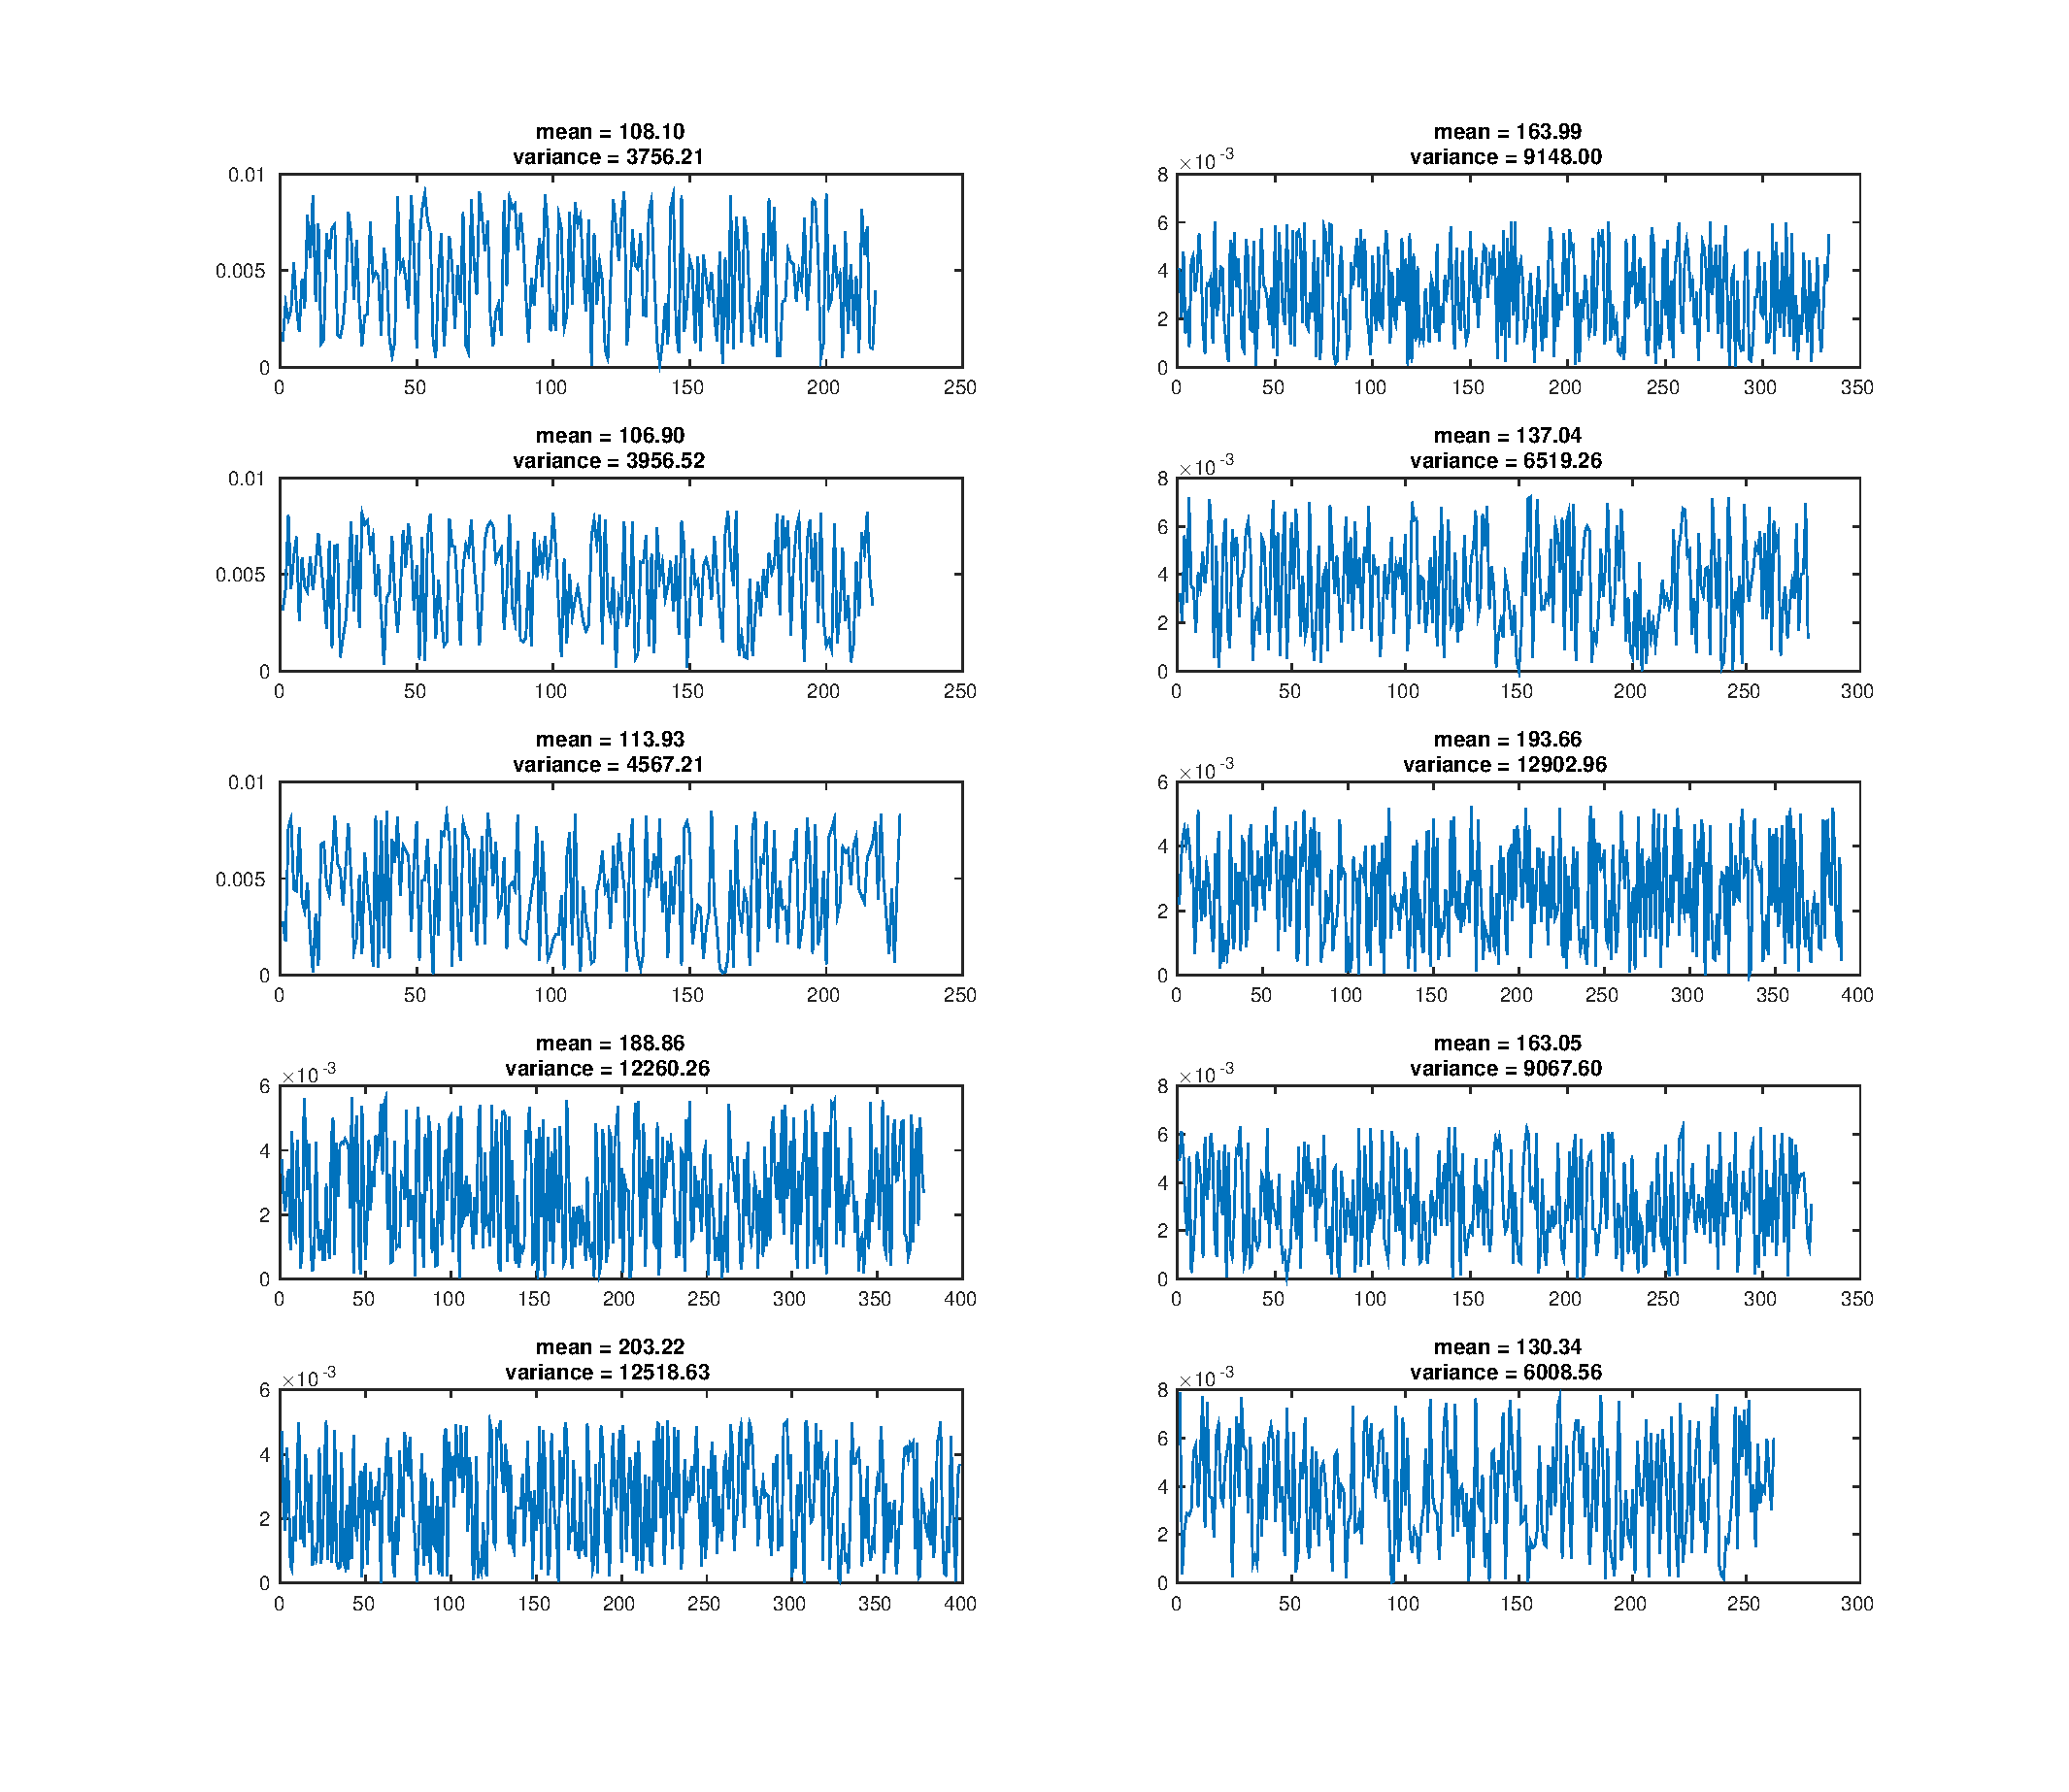
\includegraphics[width=6in]{random_distributions.eps}
    \end{center}
    \caption{Generated random distributions with their means and variances calculated.}
    \label{fig:p3a}
  \end{figure}

\item  Convolve the densities. There is a MATLAB function called \\
  \begin{center}
    \texttt{    conv;}    \\
  \end{center}
  Code segment contuned from part (a) is shown in listing~\ref{lst:p3b}
  \CodeSnippet{matlab}{Convolve all the distributions}{lst:p3b}{../src/matlab/problem3.m}{49}{70}

\item  Calculate the mean and variance of the convolution and verify the mean is the sum of the means and the variance is the sum of the variances.
  \CodeSnippet{matlab}{Code used to generate all the pics}{lst:problem3}{../src/matlab/problem3.m}{71}{79}

  outputs:
  \color{lightgray}
\begin{verbatim}
difference of mean     : 9.00
difference of variance : 0.00
\end{verbatim}
  \color{black}

\item  On the same graph, plot the convolution and the Gaussian approximation using the
  central limit theorem.
  \CodeSnippet{Matlab}{Code used to generate all the pics}{lst:problem3}{../src/matlab/problem3.m}{80}{86}
  \begin{figure}[!h]
    \begin{center}
      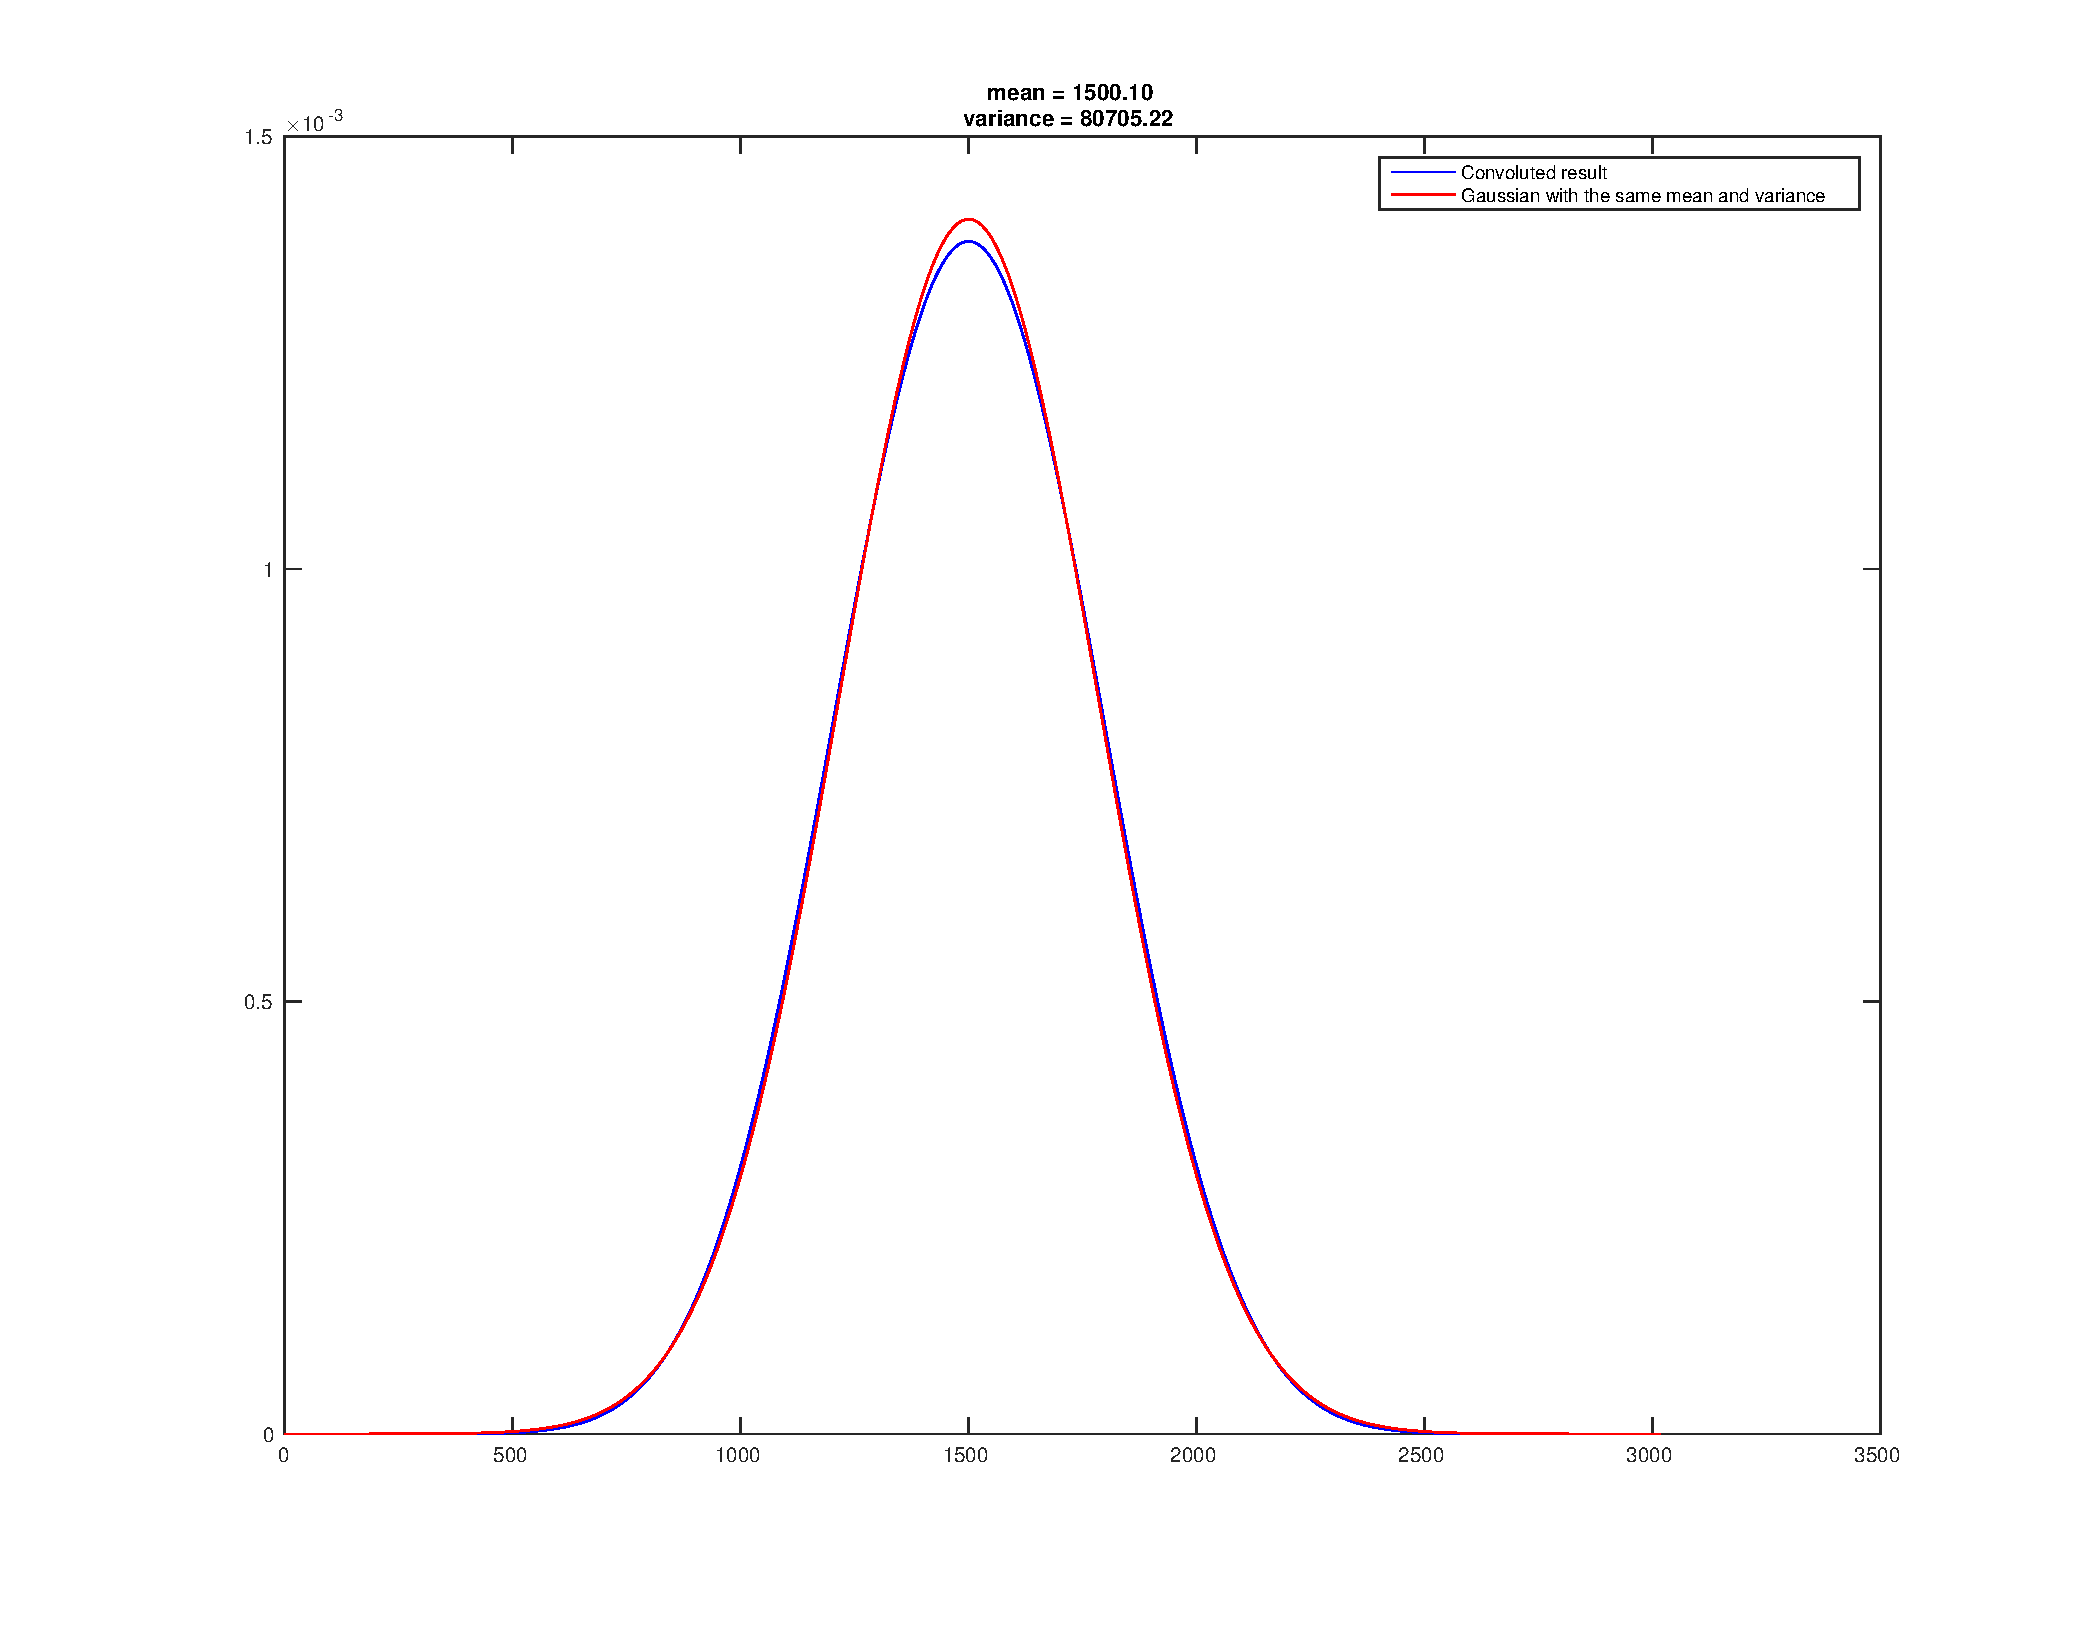
\includegraphics[width=6in]{gaussian.eps}
    \end{center}
      \caption{Convoluted distribution and gaussian pdf withe the same mean and variance}
      \label{fig:conv_gauss}
  \end{figure}
\end{enumerate}
\vspace{.5in}



\textbf{4.} Choose a probability density function other than the uniform, exponential or Laplace. 
Verify Chebyshev's inequality in equation (4.18) of the Fourier book with a computer-generated plot
\footnote{In other words, use Excel, MATLAB, or other appropriate software. Not hand drawn.}
of the inequality as a function of $a$. \\
\textbf{Solution:} \\
Chebyshev's inequality:
\begin{align*}
  \int_{\left| x - \ol{X}\leq a\right|}f_X(x)dx & \geq 1 - \left( \df{\sigma_X}{a} \right)^2
\end{align*}

In figure~\ref{fig:cheby}, blue line is a gaussian distribution with $\mu = 0, \sigma = 3$. 
Green line is a function of
\begin{align*}
  S(a) & = \int_{\ol{X} - a}^{\ol{X} + a}f_X(x)dx
\end{align*}
Red line is a function of
\begin{align*}
  Y(a) & = 1 - \left( \df{\sigma_X}{a} \right)^2
\end{align*}

The part for $-\sigma < a < \sigma$ is not shown, since they are negative.

\begin{figure}[h!]
  \begin{center}
    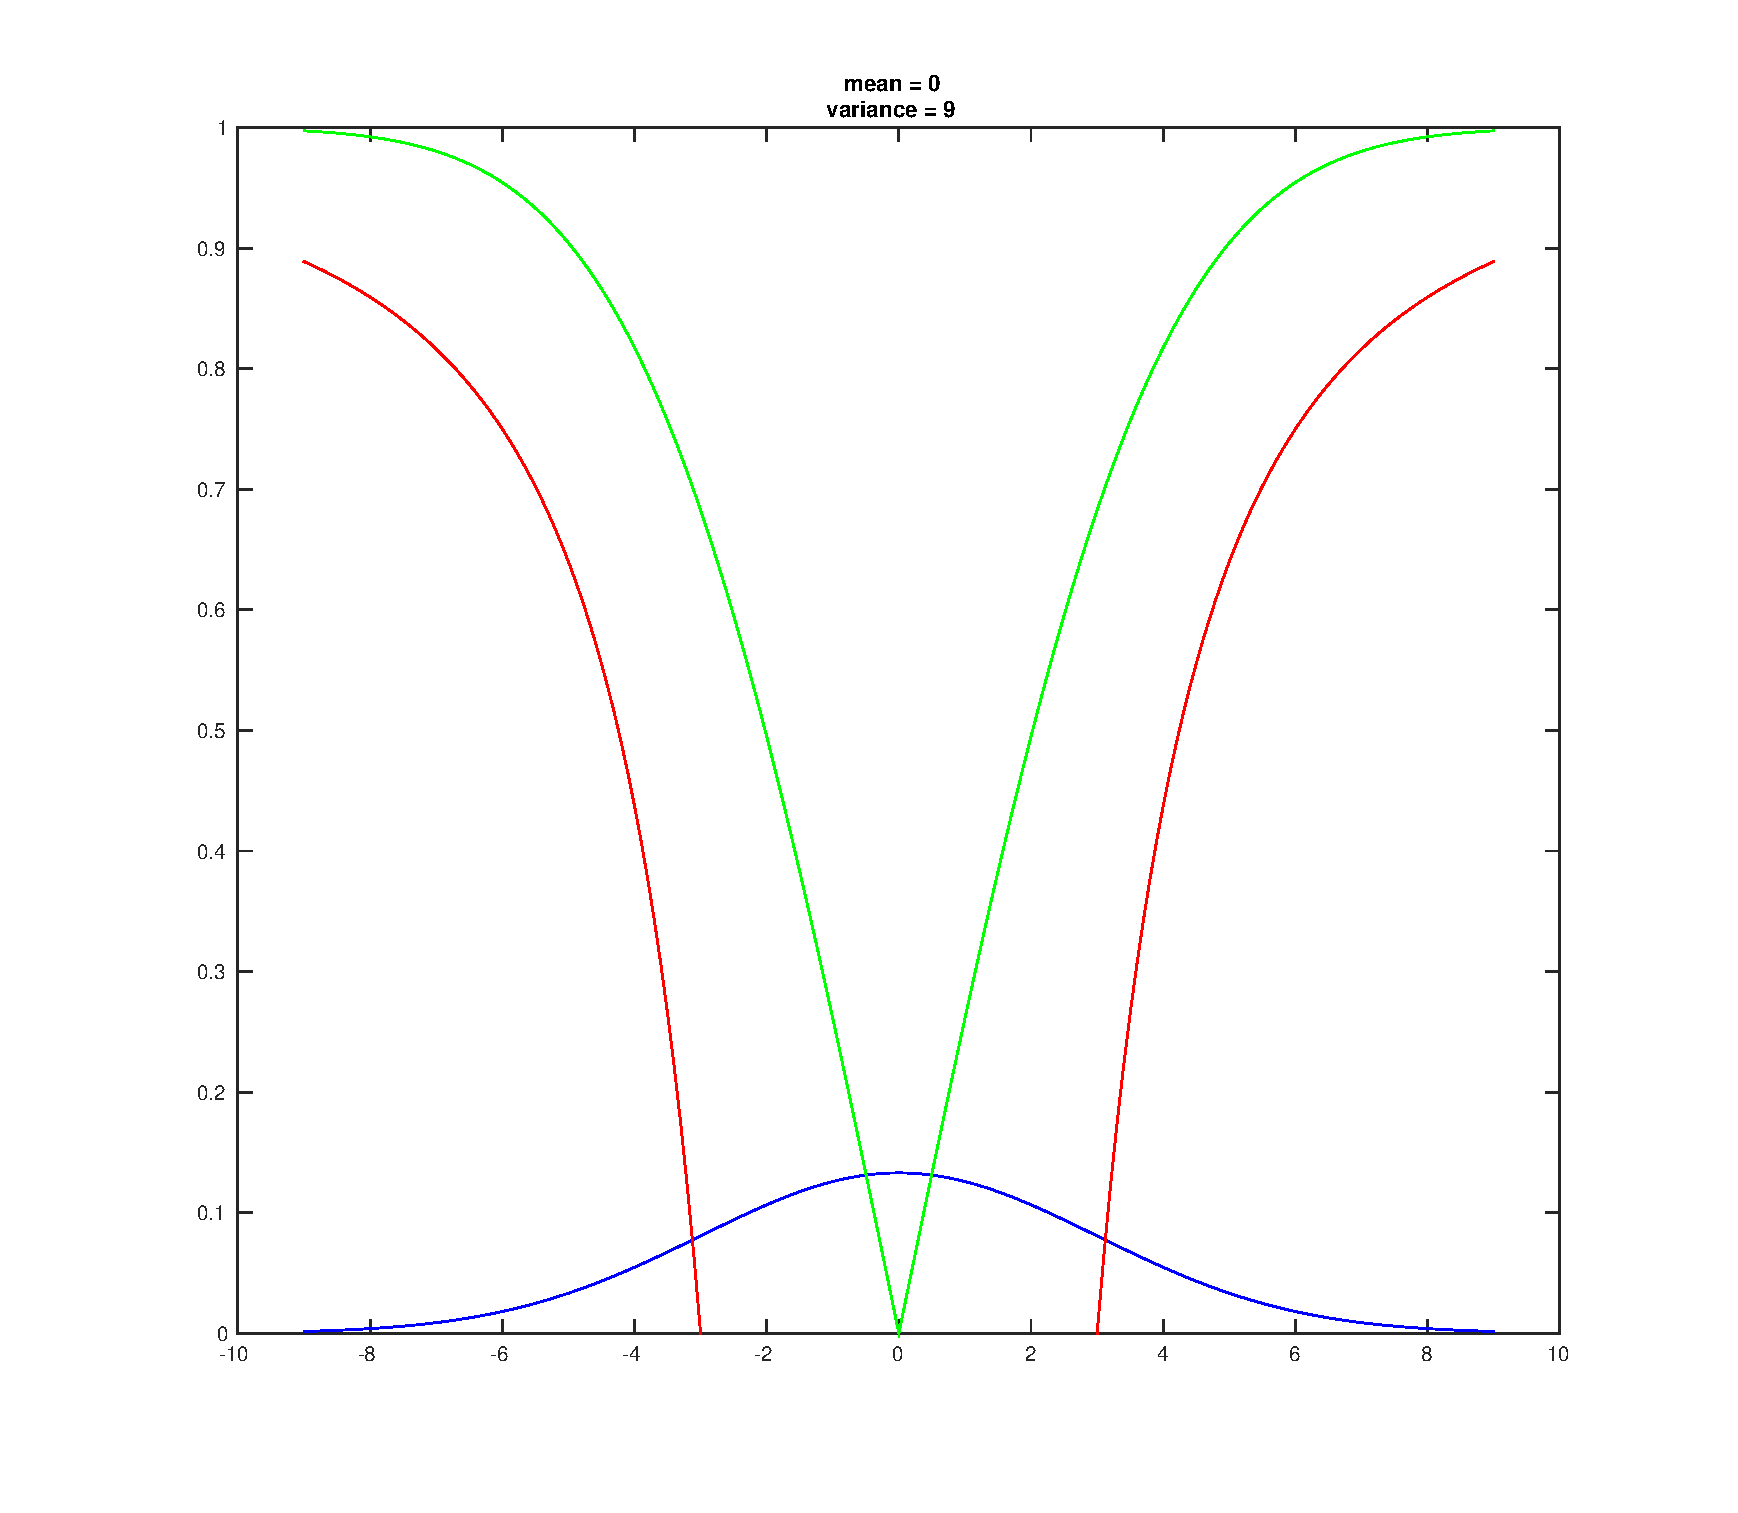
\includegraphics[width=6in]{chebyshev_inequality.eps}
  \end{center}
  \caption{Chebyshev's Inequality}
  \label{fig:cheby}
\end{figure}

\SourceCode{matlab}{Chebyshev's Inequality verification}{lst:p4}{../src/matlab/problem4.m}
\vspace{.5in}

\textbf{Old Quiz.} Here is the previous miniQuiz. If you received a perfect score of 4,
your points will be doubled. If not, you can rework the problem.
Grading is binary. Either 4 points for a correct solution or zero.

\begin{enumerate}
\item
  Let $X$ and $Y$ be i.i.d. random variables distributed as
  $$ f_X(x) = f_Y(x) = e^{-x} \mu (x)$$
  Find $f_Z (x)$ if
  \begin{enumerate}
  \item $Z=-X-Y$. \\
    \textbf{Solution:}\\
    \begin{align*}
      F_z(z) & = P\{-x-y \leq z\} = \int_{y=-\infty}^{\infty} \int_{x=-\infty}^{-z-y} f_{xy}(x, y) dx dy \\
      f_z(z) & = \df{\partial F_z(z)}{\partial z}
               = \int_{-\infty}^{\infty} \left( \df{\p}{\p z} \int_{x=-\infty}^{-z-y} f_{xy}(x, y) dx \right) dy \\
             & = - \int_{-\infty}^{\infty} f_{xy}(- z - y, y) dy
      \shortintertext{Since $x$ $y$ are independent:}
      f_{xy}(x, y) & = f_x(x)f_y(y) \\
      \shortintertext{So, we have:}
      f_z(z) & = - \int_{-\infty}^{\infty} f_x( - z -y)f_y(y) dy \\
             & = -\int_{-\infty}^{\infty} e^{-z-y}e^{y}\mu(-z -y)\mu(y) dy = 0
    \end{align*}
  \item $Z=\df{X}{Y}$
    \begin{align*}
      F_z(z) & = P\left\{ \df{x}{y} \leq z \right\}
               = P\left\{ \df{x}{y} \leq z, y > 0 \right\} + P\left\{ \df{x}{y} \leq z, y < 0 \right\} \\
             & = \int_{y=0}^{\infty} \int_{x=-\infty}^{yz} f_{xy}(x, y) dx dy
               + \int_{y=0}^{\infty} \int_{x=-\infty}^{yz} f_{xy}(x, y) dx dy \\
      f_z(z) & = \int_{0}^{\infty}yf_{xy}(yz, y) dy + \int_{-\infty}^0 -yf_{xy}(yz, y) dy \\
             & = \int_{-\infty}^{\infty} |y| f_{xy}(yz, y) dy
               = \int_{-\infty}^{\infty} |y| f_x(yz)f_y(y) dy \\
             & = \int_{-\infty}^{\infty} |y| e^{-zy}\mu(zy) e^{-y}\mu(y) dy
               = \int_{-\infty}^{\infty} |y| e^{(-z-1)y} \mu(y) dy
    \end{align*}
  \end{enumerate}
\end{enumerate}


% \begin{enumerate}
%     \item Let's assume a man wearing a boy scout leader's uniform has a son. In a conversation, you learn that he has two children.
%         \begin{enumerate}
%         \item What is the probability that the man has two sons?\footnote{
%                         Assume the chances of having a boy or a girl at 50-50.
%                          }
%             (Hint: It is not $\frac{1}{2}$.)
%         \item In addition to this information, the man says his son was born between noon and midnight.\footnote{
%                         We assume the chances of being born between noon and midnight 50-50.
%                         }
%                 Show that this additional information\footnote{
%                         If the man has two sons, we interpret this to mean that at least one of his sons was born between noon and midnight. Maybe both.
%                         }
%                  increases the probability that both of the man's sons are male.
%         \end{enumerate}

%     \item  A satellite orbits the sun such that, from the perspective of the earth, it has a period of $D$ days. Over this period, there is possible communication for $\alpha D$ days followed by $(1-\alpha ) D$ days of blackout when the sun is between the satellite and earth. The parameter $\alpha$ can be viewed as a duty cycle. Let $\lambda $ denote the average number of messages per day broadcast by the satellite. Over any time interval $T$ the number of messages broadcast by the satellite is therefore a Poisson random variable with a mean of $\lambda T $. During blackout, however, any messages transmitted by the satellite will not be received on earth.
%         \begin{enumerate}
%         \item Evaluate the probability mass function for $X=$ the number of messages received on earth in a period of $D$ days.
%         \item What is the characteristic function of $X$?
%         \item What is the mean and the variance of $X$?
%         \end{enumerate}



% \item {\bf MATLAB fun.} Digitally generate a large number of random probability density functions. An example might be\\
%         \begin{center}
%             \texttt{    S=rand(N,1);}  \\
%             \texttt{    fX=S/sum(S);} \\
%         \end{center}
%     The value or $N$ can vary for each density.
%         \begin{enumerate}
%             \item  Evaluate the mean and variance of each density.
%             \item  Convolve the densities. There is a MATLAB function called \\
%                     \begin{center}
%                     \texttt{    conv;}    \\
%                     \end{center}
%             \item  Calculate the mean and variance of the convolution and verify the mean is the sum of the means and the variance is the sum of the variances.
%             \item  On the same graph, plot the convolution and the Gaussian approximation using the
%              central limit theorem.
%         \end{enumerate}


% \item Choose a probability density function other than the uniform, exponential or Laplace. Verify Chebyshev's inequality in equation (4.18) of the Fourier book with a computer-generated plot\footnote{
%             In other words, use Excel, MATLAB, or other appropriate software. Not hand drawn.}
%     of the inequality as a function of $a$.


% \end{enumerate}


% Figure~\ref{bearz} shows how to insert a png figure.
%  \begin{figure}
%     \centering
%     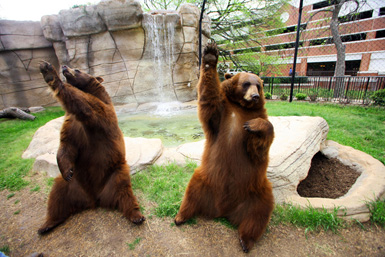
\includegraphics[width=2in]{bearz}
%     \caption{Smarter than the average bears!}
%     \label{bearz}
% \end{figure}



% \section{Mini Quizes}

% If you scored less than the maximum four points on any one of the many quizzes, you're welcome to redo the problem for full credit. This is binary. Either you will get the full credit for the mini exam from the reworked problem, or you will revert to the grade you were given on the exam. The reworked problems are due at the same time the exam is due. (I've made some teeny changes here and there.)

% If you did receive a perfect grade of four points on any many exam, your score will be doubled to eight and there is no need for you to repeat your solution here.

% \begin{enumerate}
% \item  Let $X$ by uniform on the interval (0,1). Evaluate the probability distribution function for $Y=X^a$ for $-\infty < a <\infty.$

%     {\bf Solution}:


% \item The pdf, $f_X (x)$, for an angle is uniform between 0 and $2\pi$.
%     \begin{enumerate}
%     \item What is the $\Pr [2 \leq X \leq 4]$?
%     \item Sketch and label the conditional pdf $f_X(x | 2 \leq X \leq 4)$.
%     \item Sketch and label the conditional cdf $F_X(x | 2 \leq X \leq 4)$.
%     \end{enumerate}

%     {\bf Solution}:

% \item
%     The Erlang random variable with parameters $m$, $\lambda$ and $\alpha$ is
%         \begin{equation}
%             \Phi_X (u) = \left( \frac{\alpha }{\lambda + j2\pi u}    \right)^m
%             \label{BaylorR}
%         \end{equation}
%     \begin{enumerate}
%         \item What is the value of $\alpha$ in \eqref{BaylorR}?
%                 \label{ItemMm}
%         \item What is the mean of $X$ in terms of $m$ and $\lambda$? (Use your answer in \ref{ItemMm} so that $\alpha$ does not appear in your answer.)
%         \item What is the variance of $X$ in terms of $m$ and $\lambda$?
%     \end{enumerate}

%     {\bf Solution}:

% \end{enumerate}

% \section{Extra credit}

% Generate a movie of stochastic resonance for a black-and-white image. Do separate movies with decaying memory, {\em i.e}
% $$ Y_n = (1-\alpha) X_n + \alpha Y_{n-1}$$
% for various decay factors, $0<\alpha<1$.

% This all or nothing extra credit will be due on April 1. It will count as two test problems.

\end{document}
